\todo[inline]{Verantwortlich: Jonas, Kevin}


Für den ersten Versuch mit Testpersonen wurden die Experimente zur Emotionsinduktion zu einem Gesamtexperiment verbunden. Dabei wurde darauf geachtet einen möglichst automatisierten Testablauf zu erreichen, so dass die Testperson möglichst unbeeinflusst von äußeren Reizen oder den Aktionen des Testleiters bleibt. Dazu wurde eine automatisierte Webanwendung programmiert, die der Versuchsperson alle Anweisungen und Experimente präsentiert (siehe Abbildung \ref{fig:screen_soft1}). Der Versuchsleiter wiederum kann durch eine, ebenfalls webbasierte, Kontrollkonsole Einfluss auf das Experiment nehmen, in dem er zum Beispiel den Ablauf stoppen oder Schritte überspringen kann (siehe Abbildung \ref{fig:screen_soft1}).\\

Die Ablaufkontrolle erfolgt über den Flask Webserver, der die Website darstellt. Zur Steurung können einfach URLs auf dem Server mittels einer GET bzw. POST Anfrage aufgerufen werden und so Steuerbefehle übermittelt werden. \\

Die Bilder, die dem Probanden angezeigt werden, wie auch die Spiele, die er spielen soll, sind nahtlos in die Website eingebettet. Dies ist möglich, dadurch, dass es sich zum einen um eine Javascript Anwendung und zum anderen um eine Flash Anwendung handelt. Die Flash Anwendung wurde zur einfacheren Handhabung so präpariert, dass das Menü entfernt wurde und das Spiel direkt mit dem ersten Level beim Laden startet. \\

\begin{figure}[h]
    \centering
\begin{minipage}[t]{0.9\textwidth}
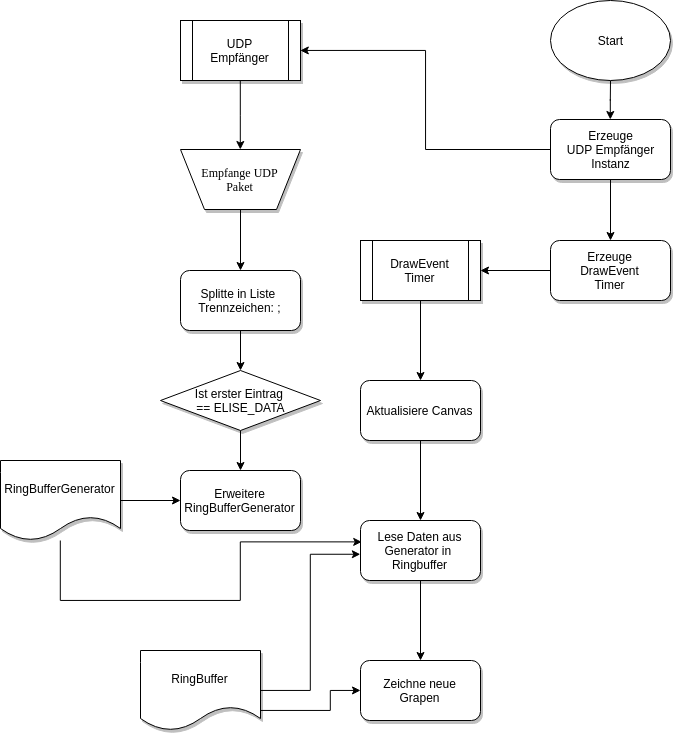
\includegraphics[width=\textwidth]{Images/ablauf_anzeige.png}
\end{minipage}
    \caption{Screenshot der Supervisor Ansicht}
    \label{fig:screen_soft1}
\end{figure}


